\documentclass[tikz,border=0mm]{standalone} 
\usetikzlibrary{positioning}
\usetikzlibrary{calc}
\usetikzlibrary{shadows.blur}
\usepackage{ifthen}
\usepackage{amsmath}
\begin{document}
\fontfamily{phv}\selectfont

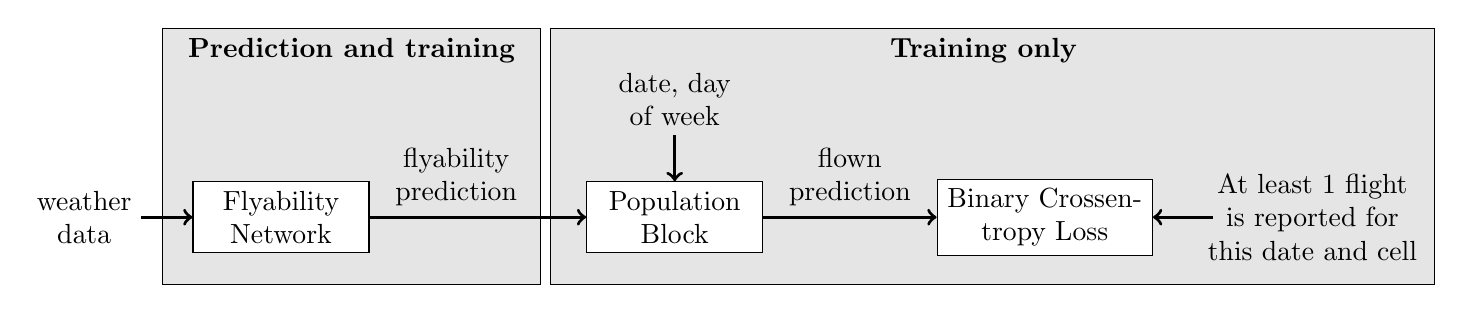
\begin{tikzpicture}

\coordinate (PBC) at (5.0cm, 0);

\draw[fill=black!10] ($(PBC)+(-6.5cm, 2.4cm)$) rectangle ($(PBC)+(-1.7cm, -0.85cm)$);
\draw[fill=black!10] ($(PBC)+(-1.58cm, 2.4cm)$) rectangle ($(PBC)+( 9.65cm, -0.85cm)$);
\node[anchor=90] at ($(PBC)+(-4.1cm, 2.4cm)$) {\textbf{Prediction and training}};
\node[anchor=90] at ($(PBC)+( 3.925cm, 2.4cm)$) {\textbf{Training only}};

\node[draw=black, fill=white, rectangle, text width=2cm, align=center] (FN) at (0,0) {Flyability Network};
\node[draw=black, fill=white, rectangle, text width=2cm, align=center] (PB) at (PBC) {Population Block};
\node[draw=black, fill=white, rectangle, text width=2.5cm, align=center] (LOSS) at (9.7cm, 0) {Binary Crossentropy Loss};

\node[align=right, text width=1.2cm, align=center] (WEATHER) at ($(FN)+(-2.5cm, 0)$) {weather data};
\node[rectangle, text width=2cm, align=center] (DATE)    at ($(PBC)+(0, 1.5cm)$) {date, day of week};
\node[rectangle, text width=3cm, align=center, outer sep=-10pt] (OUT)     at ($(LOSS)+(+3.4cm,0cm)$) {At least 1 flight is reported for this date and cell};


\draw[->, very thick] (WEATHER) -- (FN);
\draw[->, very thick] (FN) -- node[anchor=-90, pos=0.4, text width=1.9cm, align=center] {flyability prediction} (PB);
\draw[->, very thick] (PB) -- node[anchor=-90, text width=2.2cm, align=center] {flown prediction} (LOSS);
\draw[->, very thick] (OUT) -- (LOSS);
\draw[->, very thick] (DATE) -- (PB);


\end{tikzpicture}
\end{document}

